\documentclass[12pt]{jarticle}
\usepackage{TUSIreport}
\usepackage{otf}
\usepackage[dvipdfmx]{graphicx}
\usepackage[dvipdfmx]{color}
\usepackage{amsmath}
\usepackage{amssymb}
\usepackage{color}
\usepackage{hhline}
\usepackage{fancybox,ascmac}
\usepackage{multirow}
\usepackage{url}
\usepackage{bm}
\usepackage{listings,jlisting}
%%%%%%%%%%%%%%%%%%
\lstdefinestyle{py}{
    language={Python},
    backgroundcolor={\color[gray]{.85}},
    basicstyle={\small},
    identifierstyle={\small},
    commentstyle={\small\ttfamily \color[rgb]{0,0.5,0}},
    keywordstyle={\small\bfseries \color[rgb]{1,0,0}},
    ndkeywordstyle={\small},
    stringstyle={\small\ttfamily \color[rgb]{0,0,1}},
    frame={tb},
    breaklines=true,
    columns=[l]{fullflexible},
    numbers=left,
    xrightmargin=0zw,
    xleftmargin=3zw,
    numberstyle={\scriptsize},
    stepnumber=1,
    numbersep=1zw,
    morecomment=[l]{//}
}
\begin{document}
%%%%%%%%%%%%%%%%%%%%%%%%%%%%%%%%%%%%%%%%%%%%%%%%%%%%%%%%
% 表紙を出力する場合は,\提出者と\共同実験者をいれる
% \提出者{科目名}{課題名}{提出年}{提出月}{提出日}{学籍番号}{氏名}
% \共同実験者{一人目}{二人目}{..}{..}{..}{..}{..}{八人目}
%%%%%%%%%%%%%%%%%%%%%%%%%%%%%%%%%%%%%%%%%%%%%%%%%%%%%%%
\提出者{情報工学実験3}{課題2 パターン認識}
{2021}{6}{3}{4619055}{辰川力駆}
%%%%%%%%%%%%%%%%%%%%%%%%%%%%%%%%%%%%%%%%%%%%%%%%%%%%%%%%%
\共同実験者{}{}{}{}{}{}{}{}
%%%%%%%%%%%%%%%%%%%%%%%%%%%%%%%%%%%%%%%%%%%%%%%%%%%%%%%%%
% 表紙を出力する場合はコメントアウトしない
%%%%%%%%%%%%%%%%%%%%%%%%%%%%%%%%%%%%%%%%%%%%%%%%%%%%%%%%%
\表紙出力
%%%%%%%%%%%%%%%%%%%%%%%%%%%%%%%%%%%%%%%%%%%%%%%%%%%%%%%
% 以下はレポート本体,reportmain.tex に書いてある.
% \inputを使っているが,直接書いても良い.
%%%%%%%%%%%%%%%%%%%%%%%%%%%%%%%%%%%%%%%%%%%%%%%%%%%%%%%
\section{実験の要旨}
データ分析にとって必要不可欠である前処理を演習や課題を通して理解し、
Pythonを用いて実際に行うことでやり方を身に付ける。

\section{実験の目的}
演習や課題を通して、抽出や集約などの基本的なデータ前処理の仕方を理解する。

\section{実験の原理}
データ分析のためには主に、3つの前処理がある。
\begin{enumerate}
    \item 「指標、表、グラフ作成」のための前処理

          指標の計算、表やグラフに簡単に変換できるようなデータを準備することが目的である。
          必要な列 (Column) を全て持ち、
          扱いやすい単位で集約された行 (Row) が必要な範囲分存在するデータを作成する。
    \item 「教師なし学習」の入力のための前処理

          教師なし機械学習モデルに利用する説明変数を持つデータを準備することが目的である。
          1と同様なデータであるが、
          機械学習モデルの種類に応じて扱いやすいデータの型に変換したり、
          データのスケールを揃えたりする前処理が必要になる。
    \item 「教師あり学習」の入力のための前処理

          教師あり機械学習モデルに利用する学習データ、
          テストデータ、そしてモデルに適用するデータの準備をすることが目的である。
          1や2と同様の前処理だけでなく、例えば、
          複数の列を組み合わせて新たな特徴量に変換する前処理などが必要になることがある。

\end{enumerate}

こういった前処理の目的や役割があるが、
実際に前処理を進めていくにあたっての流れは、
データ構造を対象とした前処理とデータ内容を対象とした前処理に分けている。
\begin{enumerate}
    \item データ構造を対象とした前処理

          複数の行にまたがったデータ全体に及ぶ処理であり、
          前処理の中でも早い段階で実施されることが多い。
          例えば、特定のデータを抽出したり、データを結合したり、
          あるルールに従って複数の行を1行にしたりする。

    \item データ内容を対象とした前処理

          行ごとのデータの値に応じた処理で、
          行ごとに独立で処理できる。
          比較的規模の小さい処理で、
          条件を変えて繰り返されることが多い。
          例えば、
          複数の列を組み合わせて新たな列を生成したり、
          日時のデータを月毎のデータに集約したりする。
\end{enumerate}

\clearpage

\section{実験方法}
PythonをJupyter Notebook上で実行することで、今回の実験を行う。


\subsection{課題1}
reserve\_tbから$50%$の確率で顧客をサンプリングする。
サンプリングした各顧客ごとの予約件数を調査して平均を求める。
顧客のサンプリングに関して以下の2つのやり方で行う。

reserve\_tbの行を$50%$サンプリングした後に顧客を重複なく列にした場合と、
reserve\_tbから重複のない顧客の列を抽出し$50%$
サンプリングをした場合で予約件数の平均がどの様に変わるかを確認し考察する。

\subsection{課題2}
reserve\_tb、customer\_tbを使用する。
2016年1月1日から2016年12月31日までにされた
男性客による予約(reserve\_datetimeが2016-01-01から2016-12-31)の
total\_priceの最大値をホテルごとに算出する
(指定された期間に男性客による予約のなかったホテルは除外する)。
最もtotal\_priceの最大値が高かったホテルから上位10件を
ランキング形式で降順に表示する。
同じ件数の場合は同じ順位で表示する。

\subsection{課題3}
アヤメデータを実験で使ったのとは違う特徴量の組み合わせで基データ、
標準化したデータ、正規化したデータのプロットを行う。
プロットした図から読み取れることを考察する。

\subsection{課題4}
reserve\_tbを使用する。
ある顧客の予約の行にその顧客の過去90日間の予約のtotal\_priceの平均を
(total\_price\_90d)という名前の列で情報として付与する。
過去90日間に予約がなかった場合は0とする。
日にちは予約のされた日(reserve\_datetime)を基準にする。

\clearpage

\subsection{結果・検討・考察}
\subsection{課題1}
作成したプログラムは付録Aのソースコード1,2に載せた。実行結果は次のようになった。
\begin{eqnarray}
    (\text{reserve\_tb}の行を50%サンプリングした後に顧客を重複なく列にした場合)&=& 2.61010 \nonumber \\
    (\text{reserve\_tb}から重複のない顧客の列を抽出し50%サンプリングをした場合)&=& 4.69369 \nonumber
\end{eqnarray}

このような差が生まれた理由は、
サンプルされる顧客の数が違うことに原因があると考える。
後者の場合の方が顧客の数がすくなくなるので相対的に一人あたりの数が増えると考える。

\subsection{課題2}
作成したプログラムは付録Aのソースコード3に載せた。
実行結果は次の図1のようになった。
price\_maxの列を消そうか考えたが、あるほうが自然なので残した。
\begin{figure}[h]
    \begin{center}
        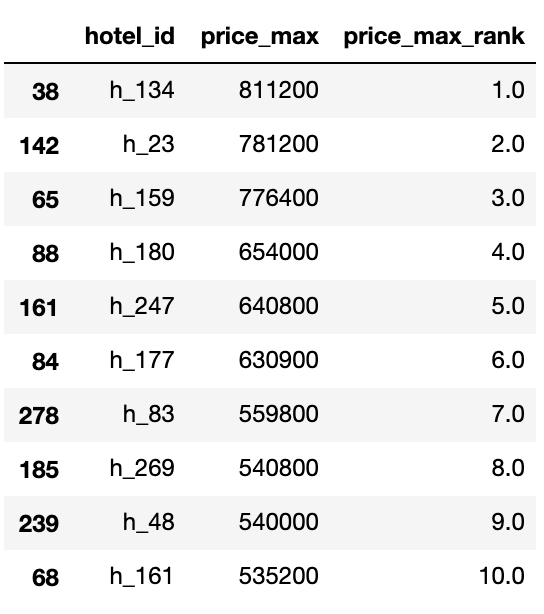
\includegraphics[scale=0.5]{kadai2_1_1.png}
    \end{center}
    \caption{課題2の結果}
\end{figure}

\clearpage
\subsection{課題3}
作成したプログラムは付録Aのソースコード4に載せた。
実行結果は次の図2のようになった。
\begin{figure}[h]
    \begin{center}
        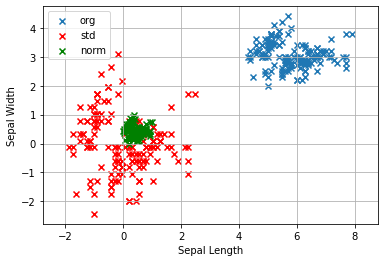
\includegraphics[scale=0.5]{kadai2_1_2.png}
    \end{center}
    \caption{課題3の結果}
\end{figure}

正規化したデータを見ると、
当たり前であるが元データを正規化したことにより
データが0から1の範囲に収まっていることが分かる。

また、どのデータを見ても分かるが、
相関はあまり強くない特徴量の組合せであることがわかる。

\subsection{課題4}
作成したプログラムは付録Aのソースコード5に載せた。
実行結果は次の図3のようになった。
\begin{figure}[h]
    \begin{center}
        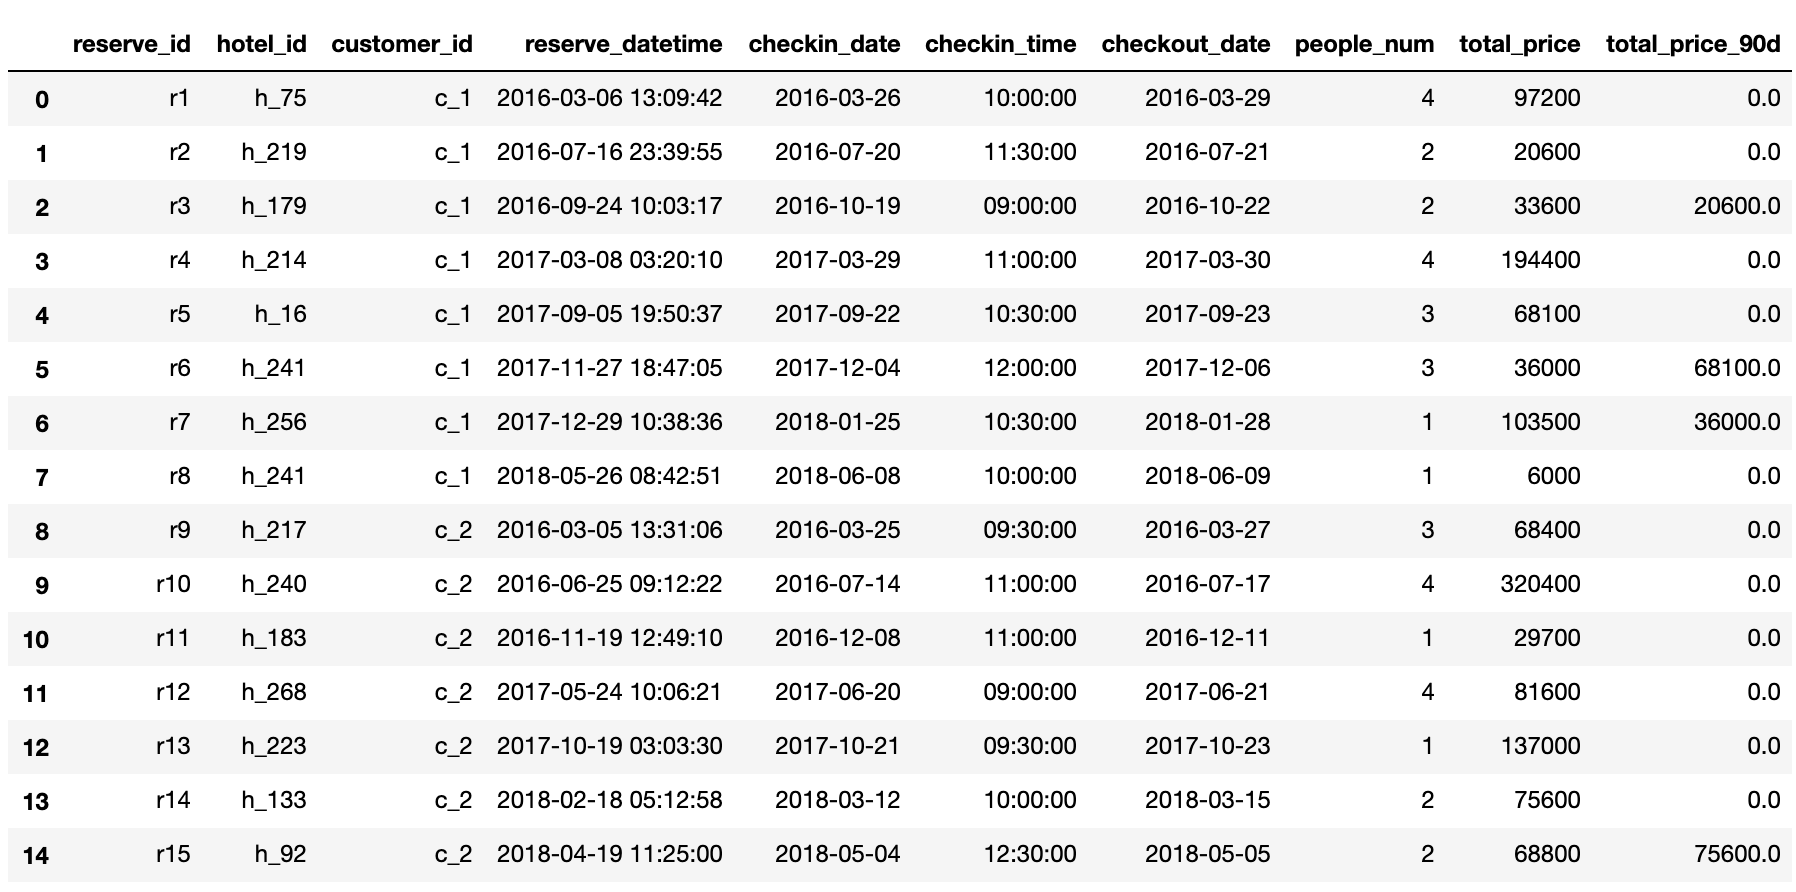
\includegraphics[scale=0.25]{kadai2_1_3.png}
    \end{center}
    \caption{課題4の結果}
\end{figure}

\clearpage
\section{まとめ}
パターン認識とは、入力データをクラス分けする処理のことであることを学んだ。
また、実際にPythonでデータ前処理を行って、
抽出や集約などの基本的なデータ前処理の仕方を理解することができた。
\clearpage
\appendix
\section{付録}

\begin{lstlisting}[style = py,caption=課題1(1)]
    ##課題1(reserve_tbの行を50%サンプリングした後に顧客を重複なく列にした場合)
    import numpy as np
    import pandas as pd
    reserve_tb = pd.read_csv('data/reserve.csv', encoding='UTF-8')
    
    reserve_tb = reserve_tb.sample(frac=0.5)
    target = reserve_tb['customer_id'].unique()
    
    kadai1_rslt = reserve_tb[reserve_tb['customer_id'].isin(target)].groupby('customer_id').size().reset_index()
    
    kadai1_rslt.columns = ['customer_id','rsv_cnt']
    
    print(kadai1_rslt['rsv_cnt'].mean())
\end{lstlisting}


\begin{lstlisting}[style = py,caption=課題1(2)]
    ##課題1(reserve_tbから重複のない顧客の列を抽出し50%サンプリングをした場合)
    import numpy as np
    import pandas as pd
    reserve_tb = pd.read_csv('data/reserve.csv', encoding='UTF-8')
    
    target = pd.Series(reserve_tb['customer_id'].unique()).sample(frac=0.5)
    kadai1_rslt = reserve_tb[reserve_tb['customer_id'].isin(target)].groupby('customer_id').size().reset_index()
    
    kadai1_rslt.columns = ['customer_id','rsv_cnt']
    
    print(kadai1_rslt['rsv_cnt'].mean())
\end{lstlisting}

\begin{lstlisting}[style = py,caption=課題2]
    ##課題2
    import numpy as np
    import pandas as pd
    reserve_tb = pd.read_csv('data/reserve.csv', encoding='UTF-8')
    customer_tb = pd.read_csv('data/customer.csv',encoding='UTF-8')
    
    kadai2_rslt = pd.merge(reserve_tb.query('"2016-01-01" <= reserve_datetime <= "2016-12-31"'),customer_tb.query('sex == "man"'),
                           on='customer_id',how='inner')
    kadai2_rslt = kadai2_rslt.groupby('hotel_id').agg({'total_price':['max']}).reset_index()
    kadai2_rslt.columns = ['hotel_id','price_max']
    kadai2_rslt['price_max_rank'] = kadai2_rslt['price_max'].rank(ascending=False,method='min')
    kadai2_rslt = kadai2_rslt.sort_values('price_max_rank', ascending=True)
    kadai2_rslt.head(10)
\end{lstlisting}

\begin{lstlisting}[style = py,caption=課題3]
    ##課題3
    import numpy as np
    import pandas as pd
    import matplotlib.pyplot as plt
    from sklearn.preprocessing import MinMaxScaler
    mmsc = MinMaxScaler()
    from sklearn.preprocessing import StandardScaler
    stdsc = StandardScaler()
    from sklearn.datasets import load_iris
    iris = load_iris()
    
    x1 = iris.data[:,0].reshape(-1,1)
    x2 = iris.data[:,1].reshape(-1,1)
    
    x=np.concatenate((x1,x2), axis=1)
    plt.axis('equal')
    plt.scatter(x[:,0],x[:,1], marker="x", label="org")
    x_norm = mmsc.fit_transform(x)
    x_std = stdsc.fit_transform(x)
    plt.scatter(x_std[:,0],x_std[:,1], c='red',marker="x", label="std")
    plt.scatter(x_norm[:,0],x_norm[:,1], c='green',marker="x", label="norm")
    plt.xlabel("Sepal Length")
    plt.ylabel("Sepal Width")
    plt.legend()
    plt.grid()
    plt.show()
\end{lstlisting}

\begin{lstlisting}[style = py,caption=課題1(2)]
    ##課題4
    import numpy as np
    import pandas as pd
    reserve_tb = pd.read_csv('data/reserve.csv', encoding='UTF-8')
    
    reserve_tb['reserve_datetime'] = pd.to_datetime(reserve_tb['reserve_datetime'])
    
    kadai4_rslt = pd.merge(reserve_tb.loc[:, ['reserve_id','customer_id','reserve_datetime']],\
                        reserve_tb.loc[:, ['customer_id','reserve_datetime', 'total_price']],on='customer_id',how='inner')
    kadai4_rslt['diffday'] = (kadai4_rslt['reserve_datetime_x'] - kadai4_rslt['reserve_datetime_y']).dt.days
    kadai4_rslt = kadai4_rslt.query('0 < diffday <= 90').groupby('reserve_id')['total_price'].mean().reset_index()
    kadai4_rslt.columns = ['reserve_id', 'total_price_90d']
    kadai4_rslt = pd.merge(reserve_tb,kadai4_rslt,on='reserve_id',how='left').fillna(0)
    kadai4_rslt.head(15)
\end{lstlisting}
%%%%%%%%%%%%%%%%%%%%%%%%%%%%%%%%%%%%%%%%%%%%%%%%%%%%%%%
\end{document}